\documentclass[border=10pt]{standalone}

\usepackage{tikz}
\usepackage{tikzsymbols}
\usetikzlibrary{calc,patterns,shapes.geometric}

\def\centerarc[#1](#2)(#3:#4:#5){\draw[#1] ($(#2)+({#5*cos(#3)},{#5*sin(#3)})$) arc (#3:#4:#5);}

\begin{document}
	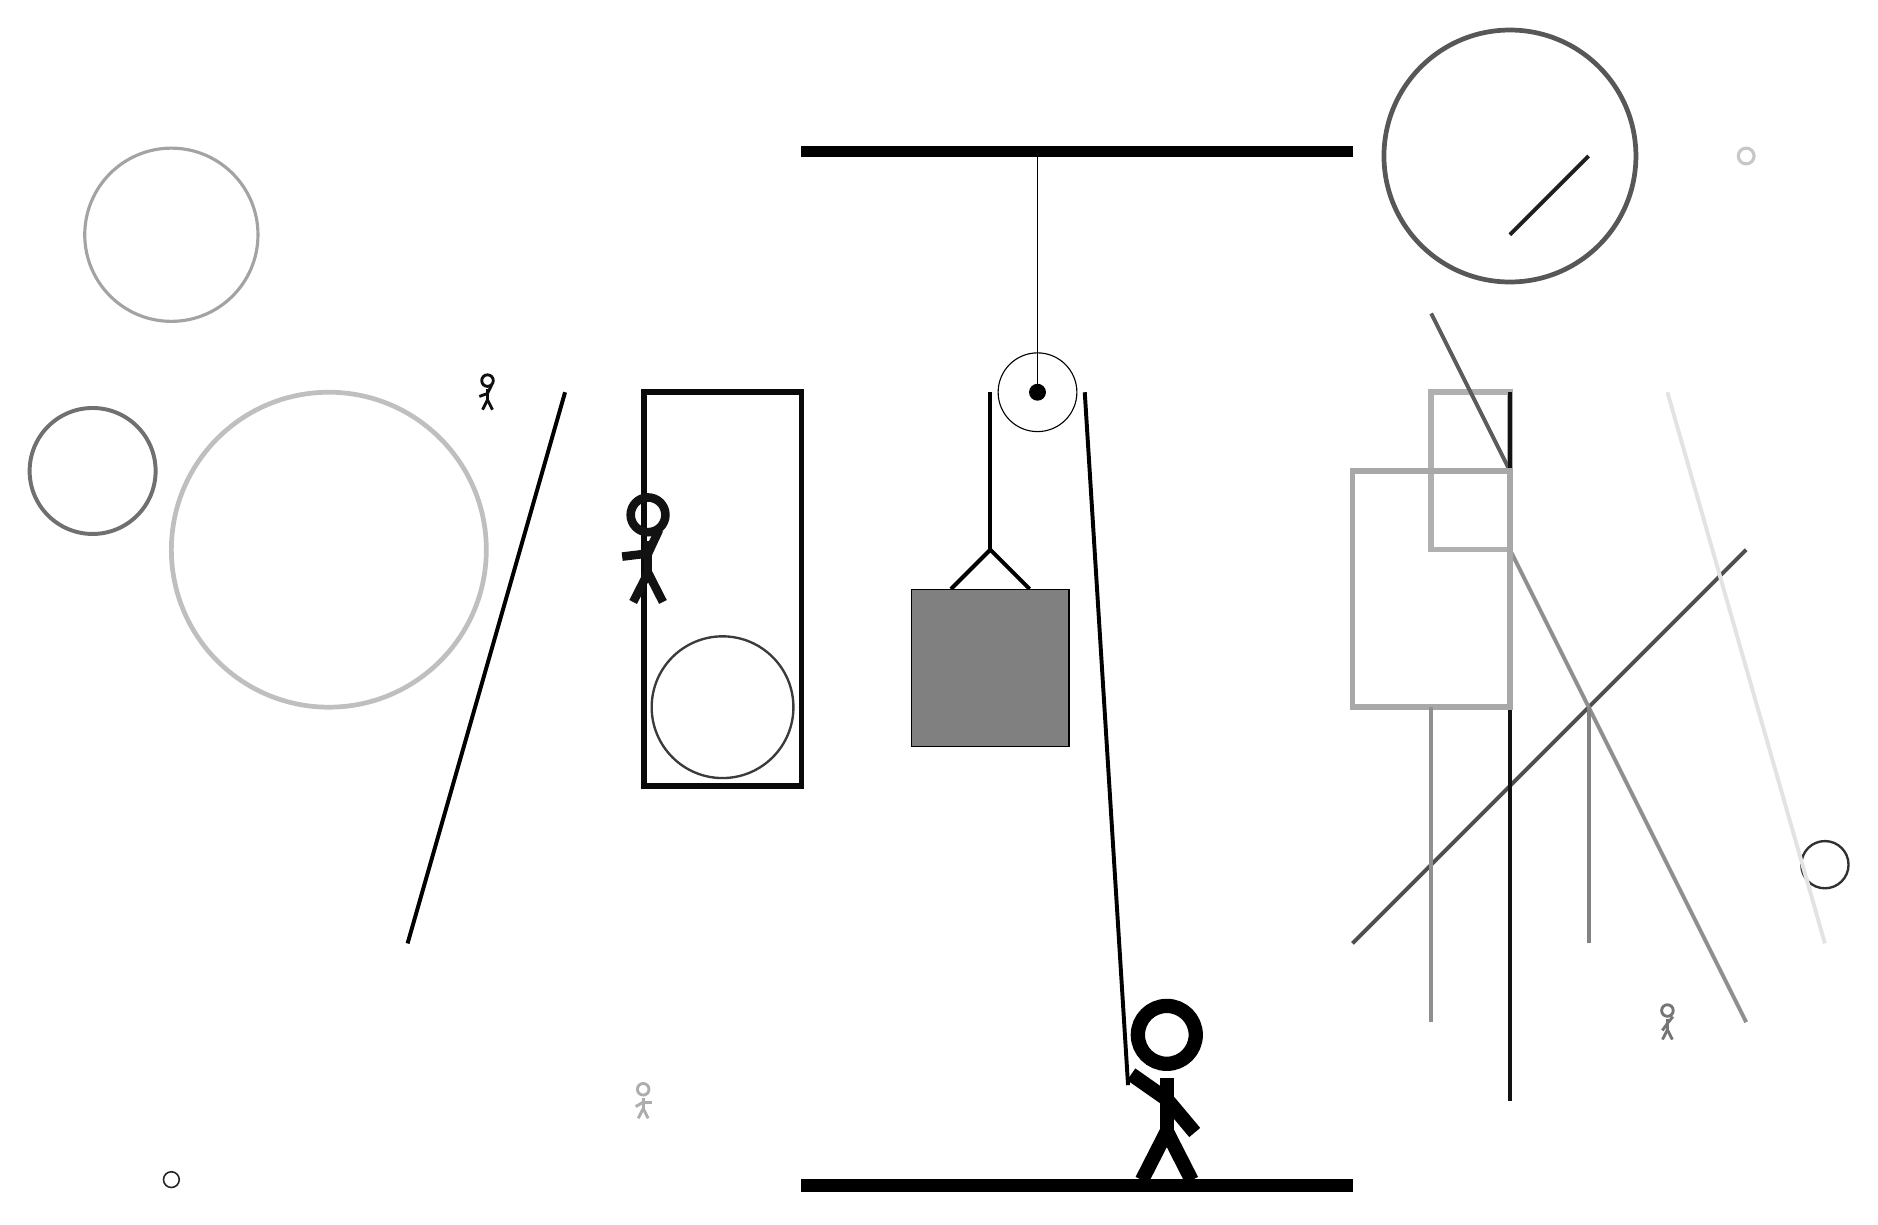
\begin{tikzpicture}
		%%%%% START %%%%%
		
		\draw[fill=black] (-2, 10) rectangle (5, 10.125);
		
		\draw (1, 7) circle (0.5);
		\draw[fill=black] (1, 7) circle (0.1);
		\draw (1, 10) -- (1, 7);
		
		\draw[line width=0.7mm, color=black!31] (6, 7) rectangle (7, 5);
		
		\draw[line width=0.5mm, color=black!100](-7, 0) -- (-5, 7);
		\draw[line width=0.5mm, color=black!69](10, 5) -- (5, 0);
		\draw [line width=0.5mm, color=black!56](-11, 6) circle (0.8);
		\draw[line width=0.5mm, color=black!64](6, 8) -- (7, 6);
		\draw[line width=0.5mm, color=black!88](7, 9) -- (8, 10);
		\draw[line width=0.5mm, color=black!44](10, -1) -- (7, 5);
		\draw [line width=0.4mm, color=black!36](-10, 9) circle (1.1);
		\draw [line width=0.6mm, color=black!66](7, 10) circle (1.6);
		\draw[line width=0.7mm, color=black!96] (-4, 7) rectangle (-2, 2);
		\draw[line width=0.4mm, color=black!93] (7, 7) rectangle (7, -2);
		\draw[line width=0.7mm, color=black!34] (7, 3) rectangle (5, 6);
		\node[line width=0.2mm, color=black!94] at (-6, 7) {\Strichmaxerl[2][20][64]};
		
		\node[line width=0.7mm, color=black!32] at (-4, -2) {\Strichmaxerl[2][31][0]};
		\draw [line width=0.3mm, color=black!81](11, 1) circle (0.3);
		\node[line width=0.4mm, color=black!54] at (9, -1) {\Strichmaxerl[2][54][51]};
		
		\draw[line width=0.5mm, color=black!49](8, 0) -- (8, 3);
		\draw[line width=0.5mm, color=black!44](6, 3) -- (6, -1);
		\draw [line width=0.6mm, color=black!25](-8, 5) circle (2.0);
		\node[line width=0.6mm, color=black!93] at (-4, 5) {\Strichmaxerl[6][7][65]};
		\draw[line width=0.5mm, color=black!11](9, 7) -- (11, 0);
		\draw [line width=0.4mm, color=black!22](10, 10) circle (0.1);
		
		\draw [line width=0.3mm, color=black!77](-3, 3) circle (0.9);
		\draw [line width=0.2mm, color=black!86](-10, -3) circle (0.1);
		
		\draw[line width=0.5mm] (-0.1, 4.5) -- (0.4, 5.0) -- (0.9, 4.5);
		\draw[fill=black!50] (-0.6, 4.5) rectangle (1.4, 2.5);
		
		\draw[line width=0.5mm] (0.4, 7) -- (0.4, 5.0);
		\centerarc[line width=0.5mm](1, 7)(0:180:0.6);
		\draw[line width=0.5mm](1.6, 7) -- (2.15, -1.8);
		
		\node at (2.6, -1.9) {\Strichmaxerl[10][-35][-50]};
		
		\draw[fill=black] (-2, -3) rectangle (5, -3.15);
		
		%%%%% END %%%%%
	\end{tikzpicture}
\end{document}